\chapter{Entalpi Reaksi}\label{ch:b2:reaction-enthalpy}

Sebuah kartrid gas kemah dipasang di bawah kompor kecil: beberapa gram
butana mendidihkan satu liter air dalam hitungan menit, dan nyala biru di
bawah panci jauh lebih panas daripada air yang mendidih. Berapa kalor yang
dilepaskan sebuah reaksi, berapa bagiannya yang sampai ke panci, dan
seberapa panas nyala itu? Tidak satu pun dari pertanyaan ini memerlukan
kompor untuk dijawab: tabel berisi beberapa bilangan untuk setiap zat, yang
diukur sekali untuk selamanya, memberikan kalor setiap reaksi yang dapat
dituliskan dengan zat-zat tersebut, pada suhu berapa pun. Bab ini
membangun pembukuan itu. Bab ini menerapkan hukum pertama termodinamika,
yang sudah dikenal dari fisika, pada sistem yang komposisinya berubah,
mendefinisikan \omterm{def:b2:reaction-enthalpy:reaction-quantity}{entalpi reaksi} sebagai turunan parsial, lalu menunjukkan
cara menghitungnya dari entalpi pembentukan, dari entalpi ikatan, dan
melalui siklus, bagaimana entalpi itu berubah terhadap suhu, serta apa
yang dikatakannya tentang nyala dan kalorimeter.

\begin{recall}
Dari fisika: hukum pertama $\Delta U = W + Q$; entalpi $H = U + pV$,
sebuah fungsi keadaan; pada tekanan luar tetap, di antara dua keadaan pada
tekanan itu, kalor yang diterima adalah $Q_p = \Delta H$; kapasitas kalor
pada tekanan tetap $C_p = (\partial H/\partial T)_p$; entalpi gas sempurna
hanya bergantung pada $T$. Jilid Tahun 1 memerikan sistem yang bereaksi
dengan kemajuan reaksinya $\xi$ dan bilangan stoikiometri $\nu_i$ dari
$0 = \sum_i\nu_i\mathrm A_i$, serta menetapkan keadaan standar setiap
spesies pada $p^\circ = \qty{1}{bar}$. Jilid sekolah (kelas 11) menyebut
sebuah reaksi \omterm{def:b2:reaction-enthalpy:exothermic}{eksoterm} jika reaksi itu melepaskan kalor, dan memperkirakan
energi pembakaran dari energi ikatan.
\end{recall}

\begin{omfigure}
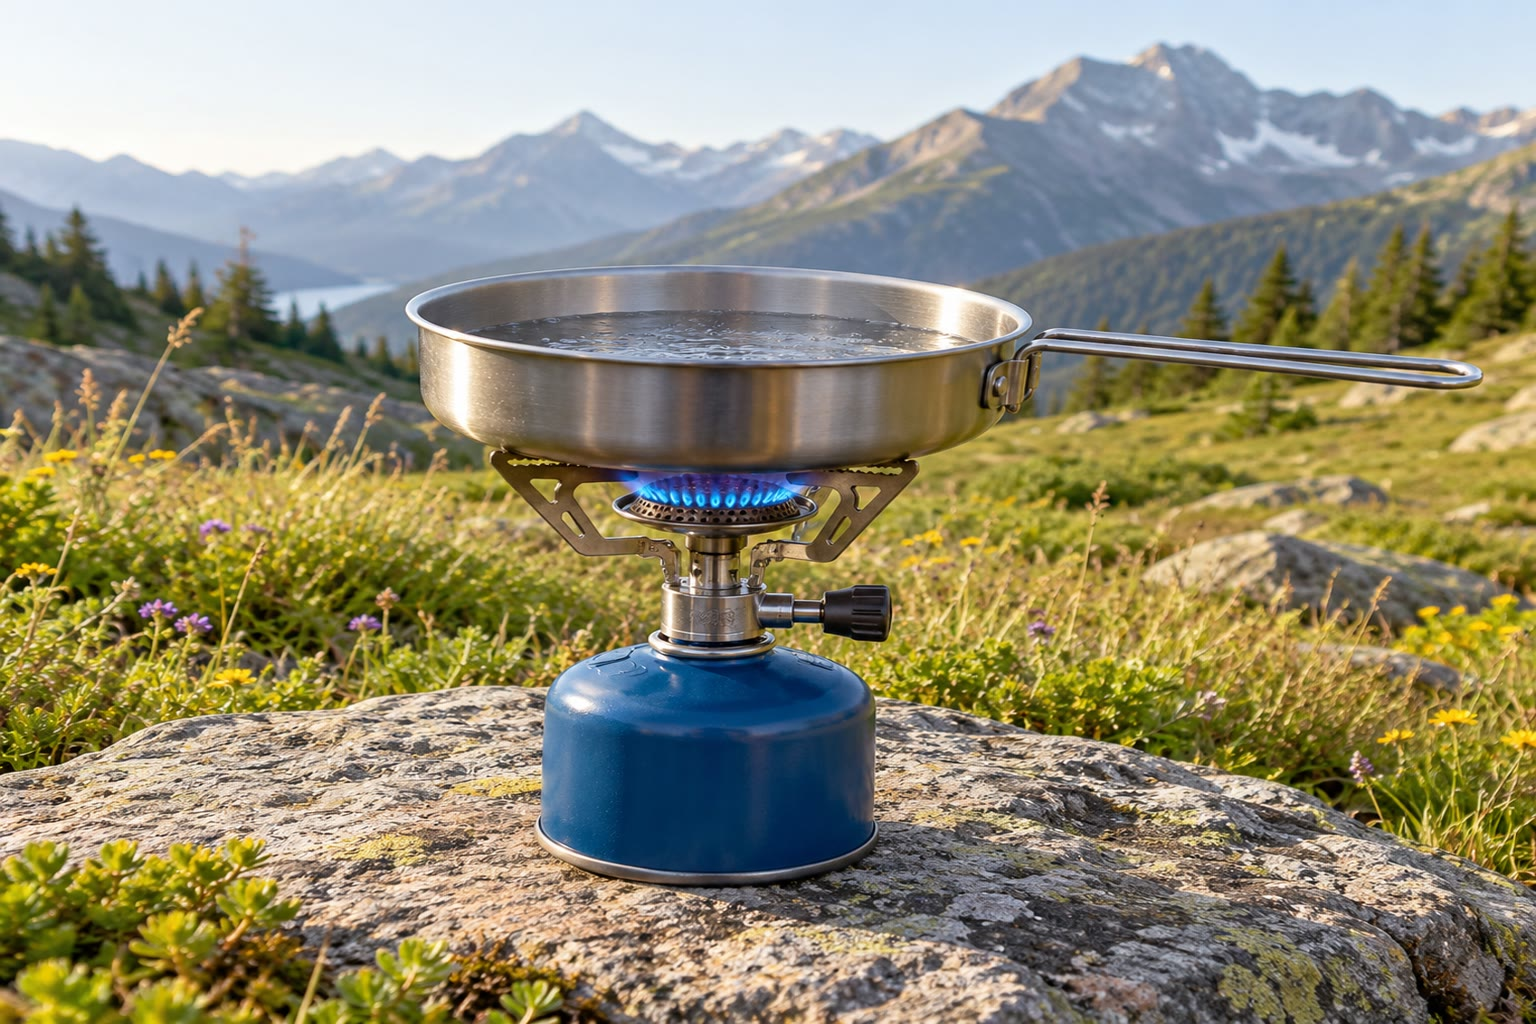
\includegraphics[width=0.6\linewidth]{images/book3/ai/b2-01-camping-stove.jpg}

{\small Sebuah kompor kemah: butana dari kartrid terbakar di udara di bawah
panci. Kalor yang dilepaskan per mol butana, bagian yang sampai ke air,
dan suhu nyala dihitung dalam soal akhir pekan bab ini.}
\end{omfigure}

\section{Besaran reaksi}

Sebuah sistem tertutup tempat berlangsungnya reaksi tunggal
$0 = \sum_i\nu_i\mathrm A_i$ diperikan oleh suhunya, tekanannya, dan
kemajuan reaksinya: jumlah zatnya adalah $n_i = n_{i,0} + \nu_i\xi$.
Dengan demikian, setiap fungsi keadaan ekstensif sistem itu, misalnya
entalpinya, merupakan fungsi $H(T, p,
\xi)$, dan diferensial totalnya
adalah
\[
  \dd H = \left(\frac{\partial H}{\partial T}\right)_{p,\xi}\dd T
        + \left(\frac{\partial H}{\partial p}\right)_{T,\xi}\dd p
        + \left(\frac{\partial H}{\partial \xi}\right)_{T,p}\dd\xi .
\]

\begin{definition}[Besaran reaksi, entalpi reaksi]\label{def:b2:reaction-enthalpy:reaction-quantity}
Untuk fungsi keadaan ekstensif $X$ dari sistem tertutup tempat
berlangsungnya reaksi $0 = \sum_i\nu_i\mathrm A_i$, yang disebut
\emph{besaran reaksi}\index{besaran reaksi} adalah turunan parsial
\[
  \Delta_r X = \left(\frac{\partial X}{\partial \xi}\right)_{T,p} ,
\]
yaitu perubahan $X$ per satuan kemajuan reaksi pada suhu dan tekanan
tetap, dalam satuan $X$ per mol. Untuk $X = H$, besaran ini adalah
\emph{entalpi reaksi}\index{entalpi reaksi} $\Delta_r H$, dalam \unit{kJ/mol}.
\end{definition}

\begin{remark}[Turunan, bukan selisih]\label{rem:b2:reaction-enthalpy:operator}
Lambang $\Delta_r$ adalah sebuah operator: operator ini bekerja pada
keadaan sistem, yang dibiarkannya tidak berubah. Menuliskan reaksi secara
lain (menggandakan koefisiennya) menggandakan $\Delta_r H$, sehingga
\omterm{def:b2:reaction-enthalpy:reaction-quantity}{besaran reaksi} tidak bermakna tanpa persamaannya. Jika entalpi molar
parsial $\bar H_i = (\partial H/\partial n_i)_{T,p,n_j}$ spesies-spesiesnya
digunakan (\cref{ch:b2:chemical-potential}), $\Delta_r H = \sum_i\nu_i\bar H_i$,
berdasarkan aturan rantai yang diterapkan pada $n_i = n_{i,0} + \nu_i\xi$.
\end{remark}

\begin{proposition}[Kalor yang diterima pada suhu dan tekanan tetap]\label{prop:b2:reaction-enthalpy:qp}
Jika reaksi maju dari $\xi_1$ ke $\xi_2$ dalam sistem yang dijaga pada
$T$ dan $p$ tetap, sistem itu menerima kalor
\[
  Q_p = \int_{\xi_1}^{\xi_2}\Delta_r H\,\dd\xi = \Delta_r H\,(\xi_2 - \xi_1)
\]
jika $\Delta_r H$ tidak bergantung pada $\xi$.
\end{proposition}

\begin{proof}
Pada $p$ tetap (dan, di sini, tekanan luar tetap), kalor yang diterima
adalah perubahan entalpi, $Q_p = \Delta H$ (fisika). Pada $T$ dan $p$
tetap, diferensial $H$ menjadi $\dd H = \Delta_r H\,\dd\xi$; integrasi
dari $\xi_1$ ke $\xi_2$ memberikan hasil tersebut.
\end{proof}

\begin{definition}[Eksoterm, endoterm, atermik]\label{def:b2:reaction-enthalpy:exothermic}
Sebuah reaksi disebut \emph{eksoterm}\index{eksoterm} pada keadaan
tertentu jika $\Delta_r H < 0$: jika berlangsung ke arah maju pada $T$ dan
$p$ tetap, reaksi itu memberikan kalor kepada lingkungan. Reaksi itu
disebut \emph{endoterm}\index{endoterm} jika $\Delta_r H >
0$, dan
\emph{atermik}\index{atermik} jika $\Delta_r H = 0$.
\end{definition}

Kalor reaksi pada umumnya tidak bergantung pada komposisi: untuk gas
sempurna serta untuk padatan dan cairan murni, entalpi setiap spesies
tidak bergantung pada apa yang ada di sekitarnya, dan $\Delta_r H$ sudah
tertentu begitu $T$ tertentu.

\begin{proposition}[Sistem ideal]\label{prop:b2:reaction-enthalpy:ideal}
Dalam campuran gas sempurna dengan fase terkondensasi murni, $\Delta_r H$
hanya bergantung pada suhu, dan sama dengan \omterm{def:b2:reaction-enthalpy:standard-reaction-enthalpy}{entalpi reaksi standar}
$\Delta_r H^\circ(T)$ yang didefinisikan di bawah. Untuk zat terlarut
dalam larutan encer, kesamaan ini berlaku dengan pendekatan yang baik.
\end{proposition}

\begin{proof}
Dalam campuran gas sempurna, setiap gas berperilaku seolah-olah sendirian,
dengan entalpi $n_iH_{m,i}(T)$ yang tidak bergantung pada $p$ (fisika:
entalpi gas sempurna hanya bergantung pada $T$). Padatan atau cairan murni
mempunyai $H = n_iH_{m,i}(T,
p)$, dan $(\partial H_m/\partial p)_T = V_m(1 - \alpha T)$ hanya beberapa \unit{J/(mol.bar)} untuk fase
terkondensasi, dapat diabaikan dibandingkan dengan \omterm{def:b2:reaction-enthalpy:reaction-quantity}{entalpi reaksi} yang
besarnya puluhan \unit{kJ/mol}. Jadi $H = \sum_in_iH_{m,i}(T)$, yang
turunannya terhadap $\xi$ adalah $\sum_i\nu_iH_{m,i}(T)$: turunan itu
hanya bergantung pada $T$, dan nilainya adalah nilai yang dihitung dengan
setiap spesies dalam keadaan standarnya.
\end{proof}

\section{Entalpi reaksi standar dan hukum Hess}

\begin{definition}[Besaran reaksi standar]\label{def:b2:reaction-enthalpy:standard-reaction-enthalpy}
Yang disebut \emph{besaran reaksi standar}\index{besaran reaksi standar}
adalah $\Delta_r X^\circ(T) = \sum_i\nu_iX_{m,i}^\circ(T)$, yaitu \omterm{def:b2:reaction-enthalpy:reaction-quantity}{besaran
reaksi} yang dihitung dengan setiap spesies dalam keadaan standarnya pada
suhu $T$, dengan $X_{m,i}^\circ$ nilai-nilai molar standarnya. Untuk
$X = H$, besaran ini adalah \emph{entalpi reaksi
standar}\index{entalpi reaksi standar} $\Delta_r H^\circ(T)$; besaran ini
hanya bergantung pada $T$.
\end{definition}

Hanya selisih entalpi yang dapat diukur, sehingga sebuah acuan dipilih
sekali untuk selamanya, sebagaimana elektrode hidrogen dipilih untuk
potensial.

\begin{definition}[Keadaan acuan standar, entalpi pembentukan standar]\label{def:b2:reaction-enthalpy:formation}
Yang disebut \emph{keadaan acuan standar}\index{keadaan acuan standar}
sebuah unsur pada suhu $T$ adalah bentuknya yang paling stabil pada $T$ di
bawah $p^\circ$: \ce{H2}, \ce{O2}, \ce{N2}, dan \ce{Cl2} sebagai gas
sempurna, karbon sebagai grafit, natrium sebagai logam, brom sebagai
cairan (pada \qty{298}{K}). Selanjutnya, \emph{entalpi pembentukan
standar}\index{entalpi pembentukan standar} $\Delta_f H^\circ$ sebuah
senyawa adalah \omterm{def:b2:reaction-enthalpy:standard-reaction-enthalpy}{entalpi reaksi standar} dari reaksi pembentukannya, yaitu
reaksi yang menghasilkan satu mol senyawa itu dari unsur-unsurnya dalam
keadaan acuannya. Berdasarkan konstruksinya, $\Delta_f H^\circ = 0$ untuk
unsur dalam keadaan acuannya.
\end{definition}

\begin{example}[Reaksi pembentukan]\label{ex:b2:reaction-enthalpy:formation}
Reaksi pembentukan air adalah \ce{H2(g) + 1/2O2(g) -> H2O(l)}, dengan
$\Delta_f H^\circ = \qty{-285.83}{kJ/mol}$ pada \qty{298.15}{K}; reaksi
pembentukan metana adalah \ce{C(s) + 2H2(g) -> CH4(g)}, $\Delta_f H^\circ =
\qty{-74.9}{kJ/mol}$; reaksi pembentukan nitrogen monoksida adalah
\ce{1/2N2(g) + 1/2O2(g) ->
NO(g)}, $\Delta_f H^\circ = \qty{+90.3}{kJ/mol}$:
senyawa \omterm{def:b2:reaction-enthalpy:exothermic}{endoterm}, yang tetap saja dihasilkan oleh gas-gas panas di dalam
mesin. Koefisien setengah tidak menjadi masalah: reaksi pembentukan adalah
alat pembukuan, bukan mekanisme.
% ledger: dfh:H2O-l, dfh:CH4_g, dfh:NO_g
\end{example}

\begin{theorem}[Hukum Hess]\label{thm:b2:reaction-enthalpy:hess}
Jika sebuah reaksi merupakan jumlah, dengan koefisien $\lambda_k$, dari
reaksi-reaksi $k$, \omterm{def:b2:reaction-enthalpy:standard-reaction-enthalpy}{entalpi reaksi standarnya} adalah kombinasi yang sama
dari \omterm{def:b2:reaction-enthalpy:standard-reaction-enthalpy}{entalpi reaksi standar} reaksi-reaksi itu:
$\Delta_r H^\circ = \sum_k\lambda_k\Delta_r H_k^\circ$
(\emph{hukum Hess}\index{hukum Hess}). Khususnya, \omterm{def:b2:reaction-enthalpy:standard-reaction-enthalpy}{entalpi reaksi standar}
dapat dihitung melalui jalur reaksi apa pun yang membawa pereaksi ke
produk.
\end{theorem}

\begin{proof}
Setiap $\Delta_r H_k^\circ = \sum_i\nu_{i,k}H_{m,i}^\circ$ linear dalam
bilangan stoikiometri. Jika reaksi itu adalah $\sum_k\lambda_k$ kali
reaksi-reaksi $k$, bilangan stoikiometrinya adalah $\nu_i = \sum_k\lambda_k
\nu_{i,k}$, dan $\Delta_r H^\circ = \sum_i\nu_iH_{m,i}^\circ = \sum_k\lambda_k
\sum_i\nu_{i,k}H_{m,i}^\circ$. Di balik aljabar ini terdapat hukum pertama:
$H$ adalah fungsi keadaan, sehingga perubahannya di antara keadaan awal
dan keadaan akhir yang sama tidak bergantung pada jalurnya.
\end{proof}

\begin{proposition}[Entalpi reaksi dari entalpi pembentukan]\label{prop:b2:reaction-enthalpy:formation-sum}
$\Delta_r H^\circ(T) = \sum_i\nu_i\,\Delta_f H_i^\circ(T)$.
\end{proposition}

\begin{proof}
Ambillah jalur yang menguraikan pereaksi menjadi unsur-unsurnya dalam
keadaan acuannya (kebalikan reaksi pembentukannya, dengan koefisien
$-\nu_i > 0$), lalu membentuk produk dari unsur-unsur yang sama (koefisien
$\nu_i > 0$). Unsur-unsur itu saling meniadakan karena persamaannya
setara, dan \omterm{thm:b2:reaction-enthalpy:hess}{hukum Hess} menjumlahkan entalpinya.
\end{proof}

\begin{omfigure}
\begin{tikzpicture}[font=\small, >={Stealth}, y=0.0062cm]
  \draw[->] (0,-1000) -- (0,180) node[above] {$H^\circ$ (\unit{kJ/mol})};
  \foreach \y in {0,-200,-400,-600,-800,-1000} \draw (-0.08,\y) -- (0.08,\y) node[left=4pt] {$\y$};
  % levels
  \draw[very thick] (1.0,0) -- (4.6,0) node[right] {\ce{C(s) + 2H2(g) + 2O2(g)}};
  \draw[very thick, omDef] (1.0,-74.9) -- (4.6,-74.9);
  \node[right, omDef] at (4.6,-110) {\ce{CH4(g) + 2O2(g)}};
  \draw[very thick, omThm] (1.0,-965.2) -- (4.6,-965.2) node[right] {\ce{CO2(g) + 2H2O(l)}};
  % arrows
  \draw[->, omDef, thick] (1.6,0) -- (1.6,-74.9);
  \node[omDef, anchor=south west, font=\footnotesize] at (1.1,5) {$\Delta_f H^\circ(\ce{CH4}) = -74.9$};
  \draw[->, omThm, thick] (3.9,0) -- (3.9,-965.2);
  \node[right, omThm, align=left] at (3.95,-500) {$\Delta_f H^\circ(\ce{CO2})$\\ $+ 2\Delta_f H^\circ(\ce{H2O})$\\ $= -965.2$};
  \draw[->, thick] (2.75,-74.9) -- (2.75,-965.2);
  \node[left, align=right] at (2.7,-650) {$\Delta_r H^\circ$\\ $= -890.3$};
\end{tikzpicture}

{\small Tingkat-tingkat entalpi pembakaran metana pada \qty{298.15}{K}.
Unsur-unsur dalam keadaan acuannya adalah titik nol. Metana terletak
\qty{74.9}{kJ/mol} di bawahnya, produk \qty{965.2}{kJ/mol} di bawahnya:
entalpi pembakaran adalah selisihnya, \qty{-890.3}{kJ/mol}, apa pun jalur
yang sebenarnya ditempuh oleh nyala.}
% ledger: dfh:CH4_g, dfh:CO2, dfh:H2O-l
\end{omfigure}

\begin{example}[Pembakaran metana]\label{ex:b2:reaction-enthalpy:methane}
Untuk \ce{CH4(g) + 2O2(g) -> CO2(g) + 2H2O(l)},
$\Delta_r H^\circ = -393.51 + 2(-285.83) - (-74.87) - 0 =
\qty{-890.3}{kJ/mol}$ pada \qty{298.15}{K}. Nilai yang diukur dalam
kalorimeter adalah \qty{-890.7}{kJ/mol}: tabel dan nyala sesuai dalam
batas ketidakpastian data. Jika air keluar sebagai uap
($\Delta_f H^\circ = \qty{-241.83}{kJ/mol}$), $\Delta_r H^\circ =
\qty{-802.3}{kJ/mol}$: selisihnya, \qty{88.0}{kJ}, adalah entalpi
penguapan dua mol air, yang diperoleh kembali oleh ketel gas dengan
mengembunkan gas buangnya.
% ledger: dfh:CO2, dfh:H2O-l, dfh:CH4_g, dch:CH4, dfh:H2O_g (computed in figdata/bachelor-2/thermo-data.py)
\end{example}

\begin{method}[Siklus Hess]\label{met:b2:reaction-enthalpy:hess-cycle}
Untuk menentukan \omterm{def:b2:reaction-enthalpy:reaction-quantity}{entalpi reaksi} yang tidak dapat diukur secara langsung:
\begin{enumerate}
  \item tuliskan reaksi sasaran beserta wujud zat-zatnya;
  \item carilah reaksi-reaksi yang entalpinya diketahui (pembakaran,
        pembentukan) yang kombinasinya, dengan koefisien $\lambda_k$,
        menghasilkan reaksi sasaran;
  \item periksalah bahwa setiap spesies yang tidak terdapat dalam reaksi
        sasaran saling meniadakan;
  \item jumlahkan entalpinya dengan koefisien yang sama.
\end{enumerate}
\end{method}

\begin{example}[Dari karbon menjadi karbon monoksida]\label{ex:b2:reaction-enthalpy:co}
Pembakaran karbon selalu menghasilkan sedikit karbon dioksida, sehingga
entalpi \ce{C(s) + 1/2O2(g) -> CO(g)} tidak dapat diukur secara langsung.
Dua pembakaran \ce{C(s) + O2(g) -> CO2(g)} ($\qty{-393.51}{kJ/mol}$) dan
\ce{CO(g) +
1/2O2(g) -> CO2(g)} ($\qty{-283.0}{kJ/mol}$, terukur) dapat
diukur; reaksi sasaran adalah reaksi pertama dikurangi reaksi kedua:
$\Delta_r H^\circ = -393.51 + 283.0 =
\qty{-110.5}{kJ/mol}$, yaitu entalpi
pembentukan karbon monoksida.
% ledger: dfh:CO2, dfh:CO_g
\end{example}

\begin{history}[Germain Henri Hess]
\begin{minipage}[t]{0.2\linewidth}\vspace{0pt}
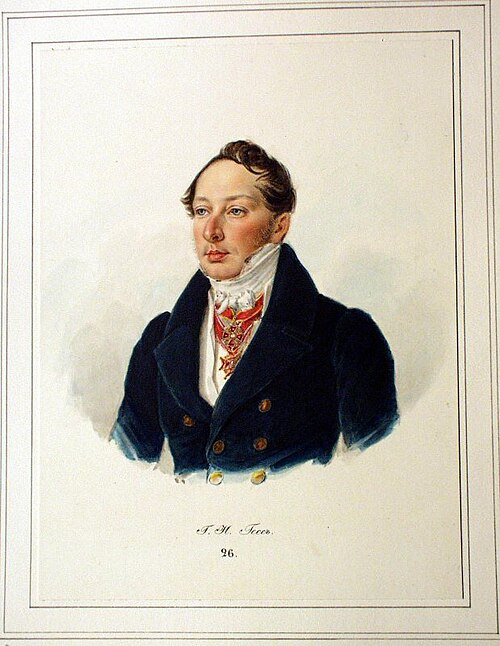
\includegraphics[width=\linewidth]{images/book3/hess.jpg}
\end{minipage}\hfill
\begin{minipage}[t]{0.76\linewidth}\vspace{0pt}
Germain Henri Hess (1802--1850), profesor kimia di Sankt-Peterburg,
mengukur kalor yang dilepaskan ketika asam sulfat diencerkan atau
dinetralkan dalam beberapa tahap, dan pada tahun 1840 mendapati bahwa
jumlahnya tidak bergantung pada tahap-tahap yang ditempuh: ``hukum
penjumlahan kalor tetap'', yang dinyatakan sebelum hukum pertama
termodinamika itu sendiri, yang menjelaskannya.
(Potret oleh I. I. Reimers, 1837--1838; CC BY-SA 4.0, Wikimedia Commons.)
\end{minipage}
\end{history}

\section{Menghitung entalpi reaksi}

\subsection*{Dari entalpi ikatan}

Jika entalpi pembentukan sebuah senyawa tidak tersedia, energi
ikatan-ikatannya memberikan perkiraan, dalam fase gas.

\begin{definition}[Entalpi disosiasi ikatan, entalpi ikatan rata-rata]\label{def:b2:reaction-enthalpy:bond-enthalpy}
Yang disebut \emph{entalpi disosiasi ikatan}\index{entalpi disosiasi ikatan}
sebuah ikatan A--B dalam molekul gas adalah \omterm{def:b2:reaction-enthalpy:standard-reaction-enthalpy}{entalpi reaksi standar}
pemutusan ikatan itu menjadi dua fragmen gas, \ce{AB(g) -> A(g) + B(g)}
untuk molekul diatomik. Jika sebuah molekul mempunyai $n$ ikatan yang
sama, \emph{entalpi ikatan rata-rata}\index{entalpi ikatan rata-rata}
molekul itu adalah entalpi standar atomisasi sempurnanya menjadi atom-atom
gas dibagi $n$.
\end{definition}

Entalpi atomisasi itu sendiri merupakan entalpi pembentukan: entalpi
pembentukan atom-atom gas dikurangi entalpi pembentukan molekulnya. Tabel
di bawah dihitung dengan cara ini.

\begin{omfigure}
\begin{tabular}{lrl}
\hline
ikatan & entalpi (\unit{kJ/mol}) & diperoleh dari \\
\hline
H--H & 436 & \ce{H2}, disosiasi \\
O=O & 498 & \ce{O2}, disosiasi \\
N$\equiv$N & 945 & \ce{N2}, disosiasi \\
Cl--Cl & 243 & \ce{Cl2}, disosiasi \\
H--Cl & 432 & \ce{HCl}, disosiasi \\
C--H & 416 & \ce{CH4}, rata-rata dari empat \\
N--H & 391 & \ce{NH3}, rata-rata dari tiga \\
O--H & 464 & \ce{H2O}, rata-rata dari dua \\
C=O & 804 & \ce{CO2}, rata-rata dari dua \\
C--C & 330 & \ce{C2H6}, dengan C--H dari metana \\
C=C & 589 & \ce{C2H4}, dengan C--H dari metana \\
\hline
\end{tabular}

\smallskip
{\small Entalpi ikatan pada \qty{298.15}{K}, dihitung dari \omterm{def:b2:reaction-enthalpy:formation}{entalpi
pembentukan standar} atom-atom dan molekul-molekul gas. Dua baris terakhir
menunjukkan batas metode ini: ikatan C--H pada etana tidak persis sama
dengan ikatan C--H pada metana, dan nilai C--C mewarisi selisihnya.}
% ledger: dfh:C_g, janaf:H, dfh:O_g, dfh:N_g, janaf:Cl, janaf:HCl, dfh:CH4_g, dfh:NH3_g, dfh:H2O_g, dfh:CO2, dfh:C2H6_g, dfh:C2H4_g (computed in figdata/bachelor-2/thermo-data.py)
\end{omfigure}

\begin{proposition}[Perkiraan dari entalpi ikatan]\label{prop:b2:reaction-enthalpy:bond-estimate}
Untuk reaksi antargas,
\[
  \Delta_r H^\circ \approx \sum(\text{entalpi ikatan yang diputus}) -
  \sum(\text{entalpi ikatan yang terbentuk}).
\]
\end{proposition}

\begin{proof}
Ikutilah jalur yang mengatomisasi setiap pereaksi (entalpinya: ikatan-ikatan
yang diputus) lalu membangun produk dari atom-atom itu (dikurangi
ikatan-ikatan yang terbentuk). \omterm{thm:b2:reaction-enthalpy:hess}{Hukum Hess} membuat jumlah ini eksak jika
setiap entalpi ikatan adalah entalpi ikatan itu dalam molekulnya sendiri;
menggantinya dengan nilai rata-rata dari molekul lain itulah pendekatannya.
\end{proof}

\begin{example}[Hidrogenasi etena]\label{ex:b2:reaction-enthalpy:hydrogenation}
Dalam \ce{C2H4(g) + H2(g) -> C2H6(g)}, satu C=C dan satu H--H diputus dan
digantikan oleh satu C--C dan dua C--H. Dengan tabel: $589 + 436 - 330 - 2
\times 416 = \qty{-137}{kJ/mol}$; dari entalpi pembentukan, nilainya
\qty{-136.3}{kJ/mol}. Kesesuaiannya baik di sini karena C--C dan C=C pada
tabel diperoleh dari molekul-molekul ini juga; untuk molekul yang tidak
mirip dengan molekul-molekul pada tabel, galat 10 sampai \qty{30}{kJ/mol}
lazim terjadi.
% ledger: dfh:C2H4_g, dfh:C2H6_g
\end{example}

\subsection*{Entalpi kisi: siklus Born--Haber}

\begin{definition}[Entalpi kisi]\label{def:b2:reaction-enthalpy:lattice-enthalpy}
Yang disebut \emph{entalpi kisi}\index{entalpi kisi} sebuah kristal ion
adalah \omterm{def:b2:reaction-enthalpy:standard-reaction-enthalpy}{entalpi reaksi standar} disosiasinya menjadi ion-ion gas: untuk
natrium klorida, \ce{NaCl(s) -> Na+(g) + Cl-(g)}. Entalpi ini bernilai
positif, dan mengukur kohesi kristal.
\end{definition}

Entalpi ini tidak dapat diukur secara langsung, tetapi sebuah siklus
melalui unsur-unsurnya memberikannya dari besaran-besaran yang dapat
diukur: entalpi pembentukan kristal, atomisasi unsur-unsurnya, energi
ionisasi logamnya, dan afinitas elektron nonlogamnya (keduanya
didefinisikan dalam jilid Tahun 1).

\begin{omfigure}
\begin{tikzpicture}[font=\small, >={Stealth}, y=0.0058cm]
  \def\lw{5.0}
  % levels (kJ/mol relative to Na(s) + 1/2 Cl2(g))
  \draw[thick] (0,0) -- (\lw,0) node[right] {\ce{Na(s) + 1/2Cl2(g)}};
  \draw[thick] (0,107.5) -- (\lw,107.5) node[right] {\ce{Na(g) + 1/2Cl2(g)}};
  \draw[thick] (0,228.8) -- (\lw,228.8) node[right] {\ce{Na(g) + Cl(g)}};
  \draw[thick] (0,724.6) -- (\lw,724.6) node[right] {\ce{Na+(g) + e- + Cl(g)}};
  \draw[thick] (0,376.1) -- (\lw,376.1) node[right] {\ce{Na+(g) + Cl-(g)}};
  \draw[thick] (0,-411.1) -- (\lw,-411.1) node[right] {\ce{NaCl(s)}};
  % the path through the elements, on the left
  \draw[->, omDef] (0.4,0) -- (0.4,107.5);
  \node[omDef, left, font=\footnotesize] at (0.35,53) {sublimasi $107.5$};
  \draw[->, omDef] (0.4,107.5) -- (0.4,228.8);
  \node[omDef, left, font=\footnotesize] at (0.35,168) {$\tfrac12$ disosiasi $121.3$};
  \draw[->, omDef] (0.4,228.8) -- (0.4,724.6);
  \node[omDef, left, font=\footnotesize] at (0.35,480) {ionisasi Na $495.8$};
  \draw[->, omThm] (1.4,724.6) -- (1.4,376.1);
  \node[omThm, right, font=\footnotesize] at (1.45,560) {penangkapan elektron $-348.6$};
  \draw[->, omProp] (2.3,0) -- (2.3,-411.1);
  \node[omProp, left, font=\footnotesize] at (2.25,-205) {pembentukan $-411.1$};
  % the lattice enthalpy, the only unknown
  \draw[->, thick] (3.6,-411.1) -- (3.6,376.1);
  \node[right, font=\footnotesize] at (3.65,-205) {entalpi kisi $787$};
\end{tikzpicture}

{\small Siklus Born--Haber natrium klorida pada \qty{298}{K}
(\unit{kJ/mol}). Naik dari kristal ke ion-ion gas melalui \omterm{def:b2:reaction-enthalpy:lattice-enthalpy}{entalpi kisi},
atau memutar melalui unsur-unsurnya, berakhir pada tingkat yang sama:
\omterm{def:b2:reaction-enthalpy:lattice-enthalpy}{entalpi kisi} adalah satu-satunya besaran yang tidak diketahui dalam siklus
ini.}
% ledger: dfh:NaCl_cr, dfh:Na_g, janaf:Cl, ie:Na, ea:Cl
\end{omfigure}

\begin{method}[Siklus Born--Haber]\label{met:b2:reaction-enthalpy:born-haber}
\begin{enumerate}
  \item Dari unsur-unsur dalam keadaan acuannya, gambarlah dua jalur: satu
        menuju kristal (pembentukan), satu menuju ion-ion gas (sublimasi
        logam, atomisasi nonlogam, ionisasi, penangkapan elektron).
  \item Tutuplah siklus itu dengan \omterm{def:b2:reaction-enthalpy:lattice-enthalpy}{entalpi kisi}, dari kristal naik ke
        ion-ion gas.
  \item Tuliskan bahwa jumlah entalpi sepanjang siklus sama dengan nol,
        lalu selesaikan untuk besaran yang tidak diketahui. Energi ionisasi
        dan afinitas elektron ditabelkan dalam eV per atom: kalikan dengan
        $N_A e = \qty{96.485}{kJ/(mol.eV)}$.
\end{enumerate}
\end{method}

\begin{example}[Natrium klorida]\label{ex:b2:reaction-enthalpy:nacl}
$\Delta_{\text{kisi}}H^\circ = 411.1 + 107.5 + 121.3 + 495.8 - 348.6 =
\qty{787}{kJ/mol}$. Energi ionisasi dan afinitas elektron adalah energi
pada \qty{0}{K}; koreksinya ke \qty{298}{K} ($+\tfrac52RT$ untuk
masing-masing) saling meniadakan di antara kedua tahap itu. Model kristal
dengan muatan titik memberikan nilai yang serupa; itulah sebabnya natrium
klorida disebut ionik.
% ledger: dfh:NaCl_cr, dfh:Na_g, janaf:Cl, ie:Na, ea:Cl (computed in figdata/bachelor-2/thermo-data.py)
\end{example}

\section{Entalpi reaksi dan suhu}

Tabel memberikan $\Delta_f H^\circ$ pada \qty{298.15}{K}. Sebuah reaktor
bekerja pada \qty{700}{K}, sebuah nyala pada \qty{2000}{K}: bagaimana
$\Delta_r H^\circ$ berubah terhadap suhu?

\begin{theorem}[Hukum Kirchhoff]\label{thm:b2:reaction-enthalpy:kirchhoff}
\[
  \frac{\dd\Delta_r H^\circ}{\dd T} = \Delta_r C_p^\circ =
  \sum_i\nu_i C_{p,m,i}^\circ ,
\]
sehingga $\Delta_r H^\circ(T_2) = \Delta_r H^\circ(T_1) + \int_{T_1}^{T_2}
\Delta_r C_p^\circ\,\dd T$ (\emph{hukum Kirchhoff}\index{hukum Kirchhoff}),
jika tidak ada perubahan wujud di antara $T_1$ dan $T_2$.
\end{theorem}

\begin{proof}
Dengan setiap spesies dalam keadaan standarnya, $H^\circ(T, \xi) = \sum_in_i
H^\circ_{m,i}(T)$ adalah fungsi dua variabel yang turunan parsial
keduanya kontinu; menurut teorema Schwarz, urutan penurunannya dapat
dipertukarkan:
\[
  \frac{\dd\Delta_r H^\circ}{\dd T} = \frac{\partial}{\partial T}
  \frac{\partial H^\circ}{\partial\xi} = \frac{\partial}{\partial\xi}
  \frac{\partial H^\circ}{\partial T} = \frac{\partial}{\partial\xi}
  \sum_in_iC^\circ_{p,m,i} = \sum_i\nu_iC^\circ_{p,m,i}.
\]
Integrasi antara $T_1$ dan $T_2$ memberikan bentuk kedua. Perubahan wujud
sebuah spesies di dalam selang itu menambahkan entalpi transisinya,
dikalikan bilangan stoikiometrinya.
\end{proof}

\begin{example}[Sintesis amonia pada suhu tinggi]\label{ex:b2:reaction-enthalpy:kirchhoff}
Untuk reaksi \ce{N2(g) + 3H2(g) -> 2NH3(g)} diketahui $\Delta_r H^\circ(298) =
\qty{-91.9}{kJ/mol}$ dan, dengan kapasitas kalor pada \qty{298}{K},
$\Delta_r C_p^\circ = 2(35.65) - 29.12 - 3(28.84) =
\qty{-44.3}{J/(K.mol)}$. Jika nilai ini dianggap tetap, diperoleh
$\Delta_r
H^\circ(700) = -91.9 - 0.0443 \times 402 = \qty{-109.7}{kJ/mol}$.
Tabel, yang mengikuti kapasitas kalor yang bertambah seiring suhu,
memberikan \qty{-105.2}{kJ/mol}: perkiraan dengan $C_p$ tetap meleset
4\,\%, harga yang wajar untuk perhitungan satu baris. Dalam rentang
\qty{400}{K}, \omterm{def:b2:reaction-enthalpy:reaction-quantity}{entalpi reaksi} berubah sekitar sepertujuhnya.
% ledger: dfh:NH3_g, cp:NH3_g.298, cp:N2_g.298, cp:H2_g.298, janafdfH:NH3.700 (computed in figdata/bachelor-2/thermo-data.py)
\end{example}

\section{Reaksi adiabatik dan kalorimetri}

\subsection*{Suhu nyala}

Dalam nyala, reaksi berlangsung cepat dan kalor tidak sempat keluar: gas-gas
itu memanaskan dirinya sendiri.

\begin{definition}[Suhu nyala adiabatik]\label{def:b2:reaction-enthalpy:flame-temperature}
Yang disebut \emph{suhu nyala adiabatik}\index{suhu nyala adiabatik}
sebuah bahan bakar adalah suhu yang dicapai oleh produk pembakaran
sempurnanya jika reaksi berlangsung pada tekanan tetap, tanpa pertukaran
kalor sama sekali, dari pereaksi pada \qty{298}{K}.
\end{definition}

\begin{proposition}[Menghitung suhu nyala]\label{prop:b2:reaction-enthalpy:flame}
Jika reaksi maju sebesar $\xi$ dari pereaksi pada $T_0$ dan sistem akhir
mempunyai kapasitas kalor $C_p(T)$, suhu akhir $T_f$ memenuhi
\[
  \xi\,\Delta_r H^\circ(T_0) + \int_{T_0}^{T_f}C_p(T)\,\dd T = 0 .
\]
\end{proposition}

\begin{proof}
Karena adiabatik dan berlangsung pada tekanan tetap, transformasi ini
mempunyai $\Delta H =
Q_p = 0$. Karena $H$ adalah fungsi keadaan, setiap
jalur di antara keadaan awal dan keadaan akhir yang sama memberikan
$\Delta H$ yang sama. Ambillah jalur pada gambar di bawah: mula-mula reaksi
pada $T_0$, dengan $\Delta H_1 = \xi\Delta_r H^\circ(T_0)$
(\cref{prop:b2:reaction-enthalpy:qp}, dengan perilaku ideal); lalu
pemanasan sistem akhir dari $T_0$ ke $T_f$, $\Delta H_2 = \int C_p\,\dd T$.
Jumlah keduanya nol.
\end{proof}

\begin{omfigure}
\begin{tikzpicture}[font=\small, >={Stealth}]
  \draw[->] (0,0) -- (6.2,0) node[right] {kemajuan $\xi$};
  \draw[->] (0,0) -- (0,3.6) node[above] {suhu $T$};
  \fill (0.6,0.6) circle (2pt) node[below left] {pereaksi, $T_0$};
  \fill (5.2,0.6) circle (2pt) node[below] {produk, $T_0$};
  \fill (5.2,3.0) circle (2pt) node[right] {produk, $T_f$};
  \draw[->, thick, omDef] (0.7,0.6) -- (5.1,0.6);
  \node[omDef, above, font=\footnotesize] at (3.15,0.64) {$\Delta H_1 = \xi\,\Delta_r H^\circ(T_0) < 0$};
  \draw[->, thick, omThm] (5.2,0.7) -- (5.2,2.9);
  \node[omThm, right, align=left] at (5.25,1.8) {$\Delta H_2 = \int_{T_0}^{T_f} C_p\,\dd T$};
  \draw[->, thick, dashed] (0.75,0.75) -- (5.05,2.92);
  \node[above left, align=center] at (2.6,1.75) {nyala nyata:\\ $\Delta H = 0$};
\end{tikzpicture}

{\small Nyala adiabatik (garis putus-putus) dan jalur setara yang terdiri
atas dua tahap: reaksi pada suhu tetap, lalu pemanasan produk. Karena $H$
adalah fungsi keadaan, jumlah perubahan entalpi kedua tahap itu sama
dengan nol.}
\end{omfigure}

\begin{method}[Suhu nyala]\label{met:b2:reaction-enthalpy:flame-temperature}
\begin{enumerate}
  \item Tuliskan pembakaran sempurna satu mol bahan bakar; di udara,
        tambahkan nitrogen dan argon yang menyertai oksigen (keduanya ikut
        dipanaskan); anggaplah air berupa uap.
  \item Hitunglah $q = -\Delta_r H^\circ(T_0)$ per mol bahan bakar.
  \item Ambillah kapasitas kalor produk $C_p$ yang tetap:
        $T_f = T_0 + q/C_p$; atau carilah $T_f$ sedemikian rupa sehingga
        jumlah kenaikan yang ditabelkan
        $n_i[H^\circ_{m,i}(T_f) - H^\circ_{m,i}(T_0)]$ sama dengan $q$,
        dengan interpolasi.
\end{enumerate}
\end{method}

\begin{omfigure}
\begin{tikzpicture}
\begin{axis}[
  width=0.8\linewidth, height=6.2cm, xmin=300, xmax=3000, ymin=0, ymax=3200,
  axis x line=bottom, axis y line=left, xlabel={$T$ (K)},
  ylabel={$H(T) - H(\qty{298}{K})$ produk (kJ)},
  xtick={500,1000,1500,2000,2500,3000},
  tick label style={font=\small}, label style={font=\small}, clip=false,
  legend style={font=\scriptsize, draw=none, at={(0.5,1.03)}, anchor=south}, legend columns=2]
\addplot[omDef, very thick] table[x=T, y=H] {figdata/out/bachelor-2-flame-temperature-butane.dat};
\addplot[omThm, very thick] table[x=T, y=H] {figdata/out/bachelor-2-flame-temperature-methane.dat};
\legend{1 mol butana di udara, 1 mol metana di udara}
\draw[omDef, dashed] (axis cs:300,2657.6) -- (axis cs:3000,2657.6);
\node[omDef, anchor=south east, font=\scriptsize] at (axis cs:2350,2657.6) {$-\Delta_r H^\circ = \qty{2657.6}{kJ}$};
\draw[omDef, dotted] (axis cs:2401,0) -- (axis cs:2401,2657.6);
\fill[omDef] (axis cs:2401,2657.6) circle (1.5pt);
\node[omDef, anchor=north west, font=\scriptsize] at (axis cs:2420,2620) {\qty{2401}{K}};
\draw[omThm, dashed] (axis cs:300,802.3) -- (axis cs:3000,802.3);
\node[omThm, anchor=south west, font=\scriptsize] at (axis cs:320,802.3) {$-\Delta_r H^\circ = \qty{802.3}{kJ}$};
\draw[omThm, dotted] (axis cs:2329,0) -- (axis cs:2329,802.3);
\fill[omThm] (axis cs:2329,802.3) circle (1.5pt);
\node[omThm, anchor=north west, font=\scriptsize] at (axis cs:2350,760) {\qty{2329}{K}};
\end{axis}
\end{tikzpicture}

{\small Entalpi yang diperlukan untuk memanaskan produk pembakaran satu
mol bahan bakar (karbon dioksida, uap air, serta nitrogen dan argon dari
udara) mulai dari \qty{298}{K}, dihitung dari entalpi yang ditabelkan.
Setiap kurva mencapai kalor yang dilepaskan oleh pembakarannya pada \omterm{def:b2:reaction-enthalpy:flame-temperature}{suhu
nyala adiabatik}: sekitar \qty{2400}{K} untuk butana, \qty{2330}{K} untuk
metana.}
% ledger: janafH:CO2.2400, janafH:H2O.2400, janafH:N2.2400, janafH:Ar.2400, air:N2, air:O2, air:Ar (computed in figdata/bachelor-2/flame-temperature.py)
\end{omfigure}

Suhu yang dihitung ini merupakan batas atas. Di atas sekitar
\qty{2000}{K}, karbon dioksida dan air mulai terdisosiasi menjadi karbon
monoksida, hidrogen, oksigen, dan radikal; reaksi-reaksi \omterm{def:b2:reaction-enthalpy:exothermic}{endoterm} ini
mengambil kembali sebagian kalor, dan nyala butana yang sesungguhnya di
udara jelas lebih dingin daripada hasil perhitungan. Dalam oksigen murni
tidak ada nitrogen yang harus dipanaskan dan nyalanya jauh lebih panas;
itulah sebabnya tukang las membakar etuna dengan oksigen, bukan dengan
udara.

\subsection*{Kalorimetri}

\begin{proposition}[Volume tetap dan tekanan tetap]\label{prop:b2:reaction-enthalpy:bomb}
Dalam bejana baja tertutup (kalorimeter bom), kalor yang diukur adalah
$Q_V =
\Delta U$, dan untuk gas sempurna serta fase terkondensasi
\[
  \Delta_r H = \Delta_r U + \Delta\nu_{\text{gas}}\,RT ,
\]
dengan $\Delta\nu_{\text{gas}}$ adalah jumlah bilangan stoikiometri
spesies-spesies gas.
\end{proposition}

\begin{proof}
$H = U + pV$, dan $\Delta_r H = \Delta_r U + \partial(pV)/\partial\xi$ pada
$T$ tetap. $pV$ fase-fase terkondensasi dapat diabaikan, dan untuk gas
$pV = n_{\text{gas}}RT$ dengan $n_{\text{gas}} = n_{\text{gas},0} +
\Delta\nu_{\text{gas}}\xi$, yang turunannya terhadap $\xi$ adalah
$\Delta\nu_{\text{gas}}RT$.
\end{proof}

\begin{omfigure}
\begin{tikzpicture}[font=\small, >={Stealth}, scale=1.0]
  % outer insulated jacket
  \draw[thick, fill=gray!8] (-2.6,-0.2) rectangle (2.6,4.4);
  \draw[thick, fill=white] (-2.3,0.1) rectangle (2.3,4.1);
  % water bath
  \fill[omDef!12] (-2.3,0.1) rectangle (2.3,3.4);
  \draw[omDef!60] (-2.3,3.4) -- (2.3,3.4);
  % bomb
  \draw[very thick, fill=gray!35] (-0.75,0.5) rectangle (0.75,2.6);
  \draw[very thick, fill=gray!55] (-0.9,2.6) rectangle (0.9,2.85);
  \draw[thick] (-0.3,1.0) -- (-0.3,1.9) (0.3,1.0) -- (0.3,1.9);
  \draw[thick, fill=orange!50] (-0.3,0.95) rectangle (0.3,1.05);
  \draw[red!70!black, thick, decorate, decoration={zigzag, amplitude=1pt, segment length=3pt}] (-0.3,1.9) -- (0.3,1.9);
  % wires
  \draw (-0.3,2.85) -- (-0.3,4.7) (0.3,2.85) -- (0.3,4.7);
  % stirrer and thermometer
  \draw[thick] (1.6,0.6) -- (1.6,4.7);
  \draw[thick, fill=gray!40] (1.35,0.55) rectangle (1.85,0.75);
  \pic[transform shape] at (-1.6,0.4) {thermometer};
  % labels
  \draw (-0.75,1.6) -- (-3.3,1.6) node[left] {bom baja, \ce{O2} pada 30 bar};
  \draw (0,1.0) -- (-3.3,0.6) node[left] {sampel dalam cawannya};
  \draw (0,1.9) -- (-3.3,2.6) node[left] {kawat penyulut};
  \draw (1.0,3.0) -- (3.3,3.0) node[right] {penangas air};
  \draw (1.6,3.9) -- (3.3,4.3) node[right] {pengaduk};
  \draw (-1.6,3.4) -- (-3.3,3.6) node[left] {termometer};
  \draw (2.45,0.3) -- (3.3,0.5) node[right] {selubung isolasi};
\end{tikzpicture}

{\small Kalorimeter bom. Sampel terbakar pada volume tetap dalam oksigen
bertekanan; kalornya masuk ke bom dan ke air yang diaduk, yang kenaikan
suhunya dibaca pada termometer. Kapasitas kalor kalorimeter ditentukan
lebih dahulu dengan membakar zat standar yang energinya diketahui.}
\end{omfigure}

\begin{method}[Kalorimetri]\label{met:b2:reaction-enthalpy:calorimetry}
\begin{enumerate}
  \item Kalibrasilah: bakar sejumlah massa zat standar yang energi
        pembakarannya diketahui (atau alirkan energi listrik yang
        diketahui), baca kenaikan suhu $\Delta T$, lalu simpulkan kapasitas
        kalor $C$ seluruh kalorimeter (air dan bejana, yang disebut
        ``setara air'' kalorimeter).
  \item Bakar sampel, baca $\Delta T'$: kalor yang dilepaskan adalah
        $C\,\Delta
        T'$, sehingga $\Delta_r U = -C\Delta T'/\xi$ pada volume
        tetap.
  \item Koreksilah ke $\Delta_r H$ dengan $\Delta\nu_{\text{gas}}RT$; dalam
        kalorimeter terbuka (tekanan tetap), langsung
        $\Delta_r H = -C\Delta T'/\xi$.
\end{enumerate}
\end{method}

\begin{example}[Sebuah pengukuran dengan bom]\label{ex:b2:reaction-enthalpy:bomb}
Untuk pembakaran butana dengan air cair, $\Delta\nu_{\text{gas}} = 4
- 1 - 6.5 = -3.5$, sehingga $\Delta_r U = \Delta_r H + 3.5RT = -2877.6 + 8.7 =
\qty{-2868.9}{kJ/mol}$: koreksinya hanya beberapa per seribu, tetapi lebih
besar daripada ketidakpastian pengukuran bom yang baik, sehingga koreksi
ini tidak pernah diabaikan.
% ledger: dfh:C4H10_g, dfh:CO2, dfh:H2O-l (computed in figdata/bachelor-2/thermo-data.py)
\end{example}

\begin{history}[Bom kalorimetri, 1881]
\begin{minipage}[t]{0.2\linewidth}\vspace{0pt}
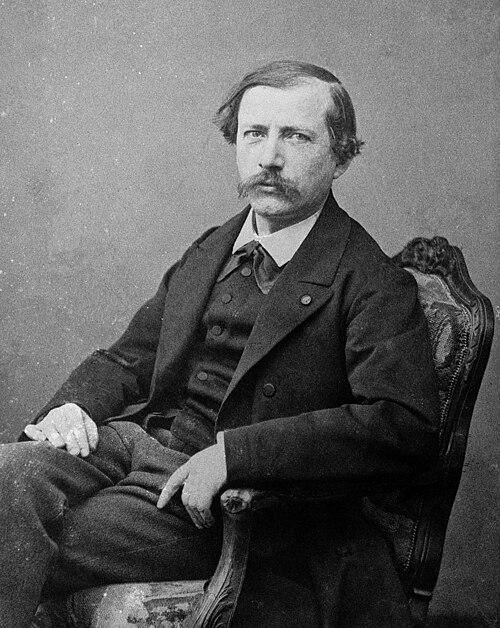
\includegraphics[width=\linewidth]{images/book3/berthelot.jpg}
\end{minipage}\hfill
\begin{minipage}[t]{0.76\linewidth}\vspace{0pt}
Marcellin Berthelot (1827--1907) membakar senyawa-senyawa organik dalam
oksigen bertekanan di dalam bejana baja tertutup berlapis platina,
sehingga pembakarannya sempurna dan tidak ada yang lolos: bom kalorimetri,
yang hingga kini masih menjadi instrumen baku untuk kalor pembakaran. Ia
juga menciptakan kata \omterm{def:b2:reaction-enthalpy:exothermic}{eksoterm} dan \omterm{def:b2:reaction-enthalpy:exothermic}{endoterm}. (Foto: domain publik,
Wikimedia Commons.)
\end{minipage}
\end{history}

\section{Latihan}

\begin{exercise}[$\star$]\label{exo:b2:reaction-enthalpy:1}
Dengan \omterm{def:b2:reaction-enthalpy:formation}{entalpi pembentukan standar} dalam bab ini, hitunglah
$\Delta_r H^\circ$ pada \qty{298}{K} untuk pembakaran propana,
\ce{C3H8(g) + 5O2(g) -> 3CO2(g) + 4H2O(l)}, jika diketahui $\Delta_f
H^\circ(\ce{C3H8}, \text{g}) = \qty{-104.7}{kJ/mol}$. Apakah reaksi itu
\omterm{def:b2:reaction-enthalpy:exothermic}{eksoterm}?
% ledger: dfh:C3H8_g
\end{exercise}

\begin{exercise}[$\star$]\label{exo:b2:reaction-enthalpy:2}
Hitunglah kalor yang dilepaskan oleh pembakaran \qty{1.00}{kg} metana (air
yang terbentuk berupa cairan) dan \qty{1.00}{kg} dihidrogen,
\ce{H2(g) + 1/2O2(g) ->
H2O(l)}. Bahan bakar manakah yang memberikan kalor
lebih banyak per kilogram?
\end{exercise}

\begin{exercise}[$\star$]\label{exo:b2:reaction-enthalpy:3}
Kalorimeter bom memberikan $\Delta_r U = \qty{-3264}{kJ/mol}$ untuk
pembakaran benzena cair menurut \ce{C6H6(l) + 15/2O2(g) -> 6CO2(g) + 3H2O(l)}
pada \qty{298}{K}. Hitunglah $\Delta_r H$.
\end{exercise}

\begin{exercise}[$\star$]\label{exo:b2:reaction-enthalpy:4}
Diketahui $\Delta_r H^\circ = \qty{-393.5}{kJ/mol}$ untuk
\ce{C(s) + O2(g) ->
CO2(g)} dan $\Delta_r H^\circ = \qty{-283.0}{kJ/mol}$
untuk \ce{CO(g) +
1/2O2(g) -> CO2(g)}. Hitunglah entalpi
\ce{CO2(g) + C(s) -> 2CO(g)}, reaksi yang berlangsung di dalam kokas panas
tanur tinggi.
\end{exercise}

\begin{exercise}[$\star\star$]\label{exo:b2:reaction-enthalpy:5}
Perkirakan, dengan entalpi ikatan dalam bab ini, entalpi
\ce{CH4(g) + Cl2(g) -> CH3Cl(g) + HCl(g)}, dengan mengambil
\qty{350}{kJ/mol} untuk C--Cl. Kemudian hitunglah besaran yang sama dari
entalpi pembentukan, jika diketahui
$\Delta_f H^\circ(\ce{CH3Cl}, \text{g}) = \qty{-83.7}{kJ/mol}$, lalu berilah
komentar tentang perbedaannya.
% ledger: dfh:CH3Cl_g
\end{exercise}

\begin{exercise}[$\star\star$]\label{exo:b2:reaction-enthalpy:6}
Entalpi penguapan standar air pada \qty{298}{K} adalah
$\Delta_f H^\circ(\ce{H2O}, \text{g}) - \Delta_f H^\circ(\ce{H2O},
\text{l})$. Hitunglah nilainya. Dengan $C_{p,m}^\circ = \qty{75.35}{J/(K.mol)}$
untuk cairan dan \qty{33.59}{J/(K.mol)} untuk uap, keduanya dianggap
tetap, perkirakan nilainya pada \qty{400}{K} (air lewat panas di bawah
tekanan), lalu bandingkan dengan tabel, yang memberikan
$\Delta_f H^\circ =
\qty{-282.59}{kJ/mol}$ untuk cairan dan
\qty{-242.85}{kJ/mol} untuk uap pada \qty{400}{K}.
% ledger: cp:H2O_l.298, cp:H2O_g.298, janafdfH:H2O_l.400, janafdfH:H2O_g.400
\end{exercise}

\begin{exercise}[$\star\star$]\label{exo:b2:reaction-enthalpy:7}
Gunakan siklus Born--Haber untuk menghitung \omterm{def:b2:reaction-enthalpy:lattice-enthalpy}{entalpi kisi} kalium klorida
dari: $\Delta_f H^\circ(\ce{KCl}, \text{s}) = \qty{-436.7}{kJ/mol}$,
sublimasi kalium \qty{89.0}{kJ/mol}, energi ionisasi kalium
\qty{4.341}{eV}, $\Delta_f H^\circ(\ce{Cl}, \text{g}) =
\qty{121.3}{kJ/mol}$,
afinitas elektron klor \qty{3.613}{eV}. Mengapa nilainya lebih kecil
daripada \omterm{def:b2:reaction-enthalpy:lattice-enthalpy}{entalpi kisi} natrium klorida?
% ledger: dfh:KCl_cr, dfh:K_g, ie:K, janaf:Cl, ea:Cl
\end{exercise}

\begin{exercise}[$\star\star$]\label{exo:b2:reaction-enthalpy:8}
Sebuah kalorimeter gelas kopi dikalibrasi dengan mengalirkan
\qty{2.00}{kJ} energi listrik, yang menaikkan suhunya sebesar
\qty{0.418}{K}. Kemudian \qty{50.0}{mL} asam klorida \qty{1.00}{mol/L}
dicampurkan di dalamnya dengan \qty{50.0}{mL} larutan natrium hidroksida
\qty{1.10}{mol/L}, keduanya pada suhu awal yang sama: suhu naik sebesar
\qty{0.583}{K}. Hitunglah entalpi \ce{H3O+(aq) + OH-(aq) ->
2H2O(l)}.
\end{exercise}

\begin{exercise}[$\star\star$]\label{exo:b2:reaction-enthalpy:9}
Oktana, model bensin, mempunyai $\Delta_f H^\circ(\text{l}) =
\qty{-250.3}{kJ/mol}$. Hitunglah entalpi pembakarannya (air berupa
cairan), kalor yang dilepaskan per kilogram, dan massa karbon dioksida
yang diemisikan per megajoule. Bandingkan dengan metana.
% ledger: dfh:C8H18
\end{exercise}

\begin{exercise}[$\star\star\star$]\label{exo:b2:reaction-enthalpy:10}
Hitunglah \omterm{def:b2:reaction-enthalpy:flame-temperature}{suhu nyala adiabatik} metana yang terbakar dalam oksigen murni
berjumlah stoikiometris, dengan kapasitas kalor tetap (nilai-nilai dalam
bab ini pada \qty{298}{K}: \ce{CO2} 37.13, \ce{H2O(g)}
\qty{33.59}{J/(K.mol)}). Bandingkan dengan hasilnya di udara,
\qty{2780}{K} dengan pendekatan yang sama. Mengapa nyala yang sesungguhnya
dalam oksigen jauh lebih dingin daripada yang dinyatakan perhitungan ini?
% ledger: cp:CO2_g.298, cp:H2O_g.298
\end{exercise}

\begin{exercise}[$\star\star\star$]\label{exo:b2:reaction-enthalpy:11}
Kapasitas kalor sebuah gas sering dituliskan $C_{p,m}^\circ = a + bT$.
Untuk sintesis amonia, ambillah $\Delta_r a = \qty{-60.5}{J/(K.mol)}$ dan
$\Delta_r b = \qty{0.0540}{J/(K^2.mol)}$ (dicocokkan dengan tabel antara
\qty{300}{K} dan \qty{800}{K}). Integrasikan \omterm{thm:b2:reaction-enthalpy:kirchhoff}{hukum Kirchhoff} dari
\qty{298}{K} sampai \qty{700}{K}, lalu bandingkan dengan nilai dalam
tabel, \qty{-105.2}{kJ/mol}, dan dengan perkiraan $C_p$ tetap.
\end{exercise}

\begin{exercise}[$\star\star\star$]\label{exo:b2:reaction-enthalpy:12}
Nitrogen monoksida terbentuk di dalam mesin melalui
\ce{N2(g) + O2(g) -> 2NO(g)}. Hitunglah \omterm{def:b2:reaction-enthalpy:standard-reaction-enthalpy}{entalpi reaksi standarnya} pada
\qty{298}{K}. Tunjukkan bahwa, jika $\Delta_r C_p^\circ$ kecil, reaksi
itu menyerap kalor yang kira-kira sama pada \qty{2000}{K}; dengan
kapasitas kalor dari tabel pada \qty{298}{K} (\ce{NO}
\qty{29.85}{J/(K.mol)}, \ce{N2} 29.12, \ce{O2} \qty{29.38}{J/(K.mol)}),
perkirakan perubahannya antara \qty{298}{K} dan \qty{2000}{K}. Jelaskan
mengapa sebuah reaksi \omterm{def:b2:reaction-enthalpy:exothermic}{endoterm} justru dapat menjadi masalah pada nyala
yang paling panas.
% ledger: dfh:NO_g, cp:NO_g.298, cp:N2_g.298, cp:O2_g.298
\end{exercise}

\section{Soal: Kartrid Gas Kemah}

\begin{problem}[{Soal akhir pekan --- energi butana, pengukuran dalam
kalorimeter bom, air yang dipanaskan dalam panci, dan suhu nyala}]
\label{pb:b2:reaction-enthalpy:1}
Sebuah kompor kemah membakar butana dari kartrid berisi \qty{230}{g}.
Data pada \qty{298}{K} ($\Delta_f H^\circ$ dalam \unit{kJ/mol}):
\ce{C4H10(g)} $-125.6$, \ce{CO2(g)} $-393.51$, \ce{H2O(l)} $-285.83$,
\ce{H2O(g)} $-241.83$. Massa molar: \ce{C4H10} \qty{58.12}{g/mol},
\ce{H2O} \qty{18.02}{g/mol}. Kapasitas kalor air cair
\qty{75.35}{J/(K.mol)}. Udara kering: \qty{20.95}{\percent} \ce{O2},
\qty{78.08}{\percent} \ce{N2}, \qty{0.93}{\percent} \ce{Ar} menurut
volume. $R = \qty{8.314}{J/(K.mol)}$.
% ledger: dfh:C4H10_g, dfh:CO2, dfh:H2O-l, dfh:H2O_g, cp:H2O_l.298, air:O2, air:N2, air:Ar

\medskip
\noindent\textbf{Bagian I --- Bahan bakar.}
\begin{enumerate}
  \item Tuliskan pembakaran sempurna butana, dengan air yang terbentuk
        berupa cairan, untuk satu mol butana.
  \item Hitunglah \omterm{def:b2:reaction-enthalpy:standard-reaction-enthalpy}{entalpi reaksi standarnya} pada \qty{298}{K}.
  \item Hitunglah sekali lagi dengan air yang terbentuk berupa uap, lalu
        jelaskan perbedaannya.
  \item Hitunglah kalor yang dilepaskan per gram butana dalam setiap kasus.
  \item Manakah dari kedua nilai itu yang memerikan kompor kemah, yang
        airnya meninggalkan nyala sebagai uap?
  \item Berapa kalor yang dapat dilepaskan oleh seluruh kartrid pada
        kompor itu?
\end{enumerate}

\medskip
\noindent\textbf{Bagian II --- Sebuah pengukuran.}
Sampel \qty{0.500}{g} butana dibakar dalam kalorimeter bom yang kapasitas
kalornya \qty{10.00}{kJ/K}; air yang terbentuk mengembun.
\begin{enumerate}[resume]
  \item Besaran apa yang diukur oleh kalorimeter bom, dan mengapa?
  \item Hitunglah $\Delta\nu_{\text{gas}}$ reaksi pada pertanyaan 1.
  \item Hitunglah $\Delta_r U$ yang diharapkan.
  \item Hitunglah kenaikan suhu kalorimeter yang diharapkan.
  \item Kenaikan yang terbaca adalah \qty{2.461}{K}. Simpulkan
        $\Delta_r U$ dan $\Delta_r H$ yang terukur, serta selisih relatifnya
        terhadap tabel.
\end{enumerate}

\medskip
\noindent\textbf{Bagian III --- Panci.}
\begin{enumerate}[resume]
  \item Hitunglah kalor yang diperlukan untuk memanaskan \qty{1.00}{L} air
        (\qty{1.00}{kg}) dari \qty{20}{\celsius} sampai \qty{100}{\celsius}.
  \item Kompor melakukannya dengan \qty{16.0}{g} butana. Hitunglah
        efisiensinya (kalor yang diterima air dibagi kalor yang
        dilepaskan).
  \item Ke mana perginya sisa kalor itu?
  \item Berapa liter air yang dapat dididihkan oleh seluruh kartrid
        dengan efisiensi ini?
\end{enumerate}

\medskip
\noindent\textbf{Bagian IV --- Nyala.}
\begin{enumerate}[resume]
  \item Butana terbakar dalam udara berjumlah stoikiometris. Hitunglah
        jumlah dinitrogen dan argon yang menyertai dioksigen yang
        diperlukan oleh satu mol butana.
  \item Tuliskan daftar jumlah produk, termasuk nitrogen dan argon.
  \item Jelaskan, dengan jalur dua tahap, mengapa kalor yang dilepaskan
        reaksi pada \qty{298}{K} (air berupa uap) seluruhnya dipakai untuk
        memanaskan gas-gas ini.
  \item Dengan kapasitas kalor pada \qty{298}{K}, \ce{CO2} 37.13,
        \ce{H2O(g)} 33.59, \ce{N2} 29.12, \ce{Ar} \qty{20.79}{J/(K.mol)},
        hitunglah kapasitas kalor produk.
  \item Simpulkan suhu nyala dengan kapasitas kalor tetap.
  \item Kenaikan entalpi dari tabel memberikan, untuk produk satu mol
        butana, \qty{2515.7}{kJ} antara \qty{298}{K} dan \qty{2300}{K},
        dan \qty{2655.7}{kJ} antara \qty{298}{K} dan \qty{2400}{K}.
        Tentukan suhu nyala dengan interpolasi linear.
  \item Mengapa perkiraan pertama terlalu tinggi?
  \item Mengapa suhu terukur nyala butana bahkan lebih rendah lagi?
  \item Nyatakan \omterm{def:b2:reaction-enthalpy:flame-temperature}{suhu nyala adiabatik} butana di udara.
\end{enumerate}
\end{problem}
